%\documentclass[mathserif, aspectratio=169]{intbeamer}
\documentclass[mathserif,aspectratio=169]{beamer}
\usepackage[utf8]{inputenc}
\usepackage[english]{babel}
\usepackage{subcaption}
\captionsetup[subfigure]{skip=2pt} % global setting for subfigure
\usepackage{amsmath,amssymb,amsfonts}
\usepackage{trfsigns}
%\usepackage{gensymb}
%\usepackage{macros}
\usepackage{xcolor}
%\usepackage{enumerate}
\setbeamercovered{invisible}
\usepackage{tikz}
\usetikzlibrary{calc}
\usepackage{comment}

\includecomment{plottikz}
%\excludecomment{plottikz}
\definecolor{pyplotC0}{RGB}{31,119,180}

\newcommand{\tw}{0.73}

% ===== titlepage info =====
\title[Shelving Filter with Adjustable Transition Band]%
{Shelving Filter Cascade with Adjustable\\Transition Slope and Bandwidth}

\author[Schultz, Hahn, Spors]{%
    \underline{Frank Schultz}, Nara Hahn, Sascha Spors}

\date[2020 June 2-5 ]{%\raisebox{0mm}{\includegraphics[width=4.6cm]{logo.png}}\\
  148th AES Convention Vienna 2020}

\institute[]{Research Group Signal Processing and Virtual Acoustics,
University of Rostock}

\begin{document}
\maketitle
%
%
%
\section{Motivation}
\begin{frame}{Low Order Shelving Filter Design}
\begin{figure}
\captionsetup{width=.75\linewidth}
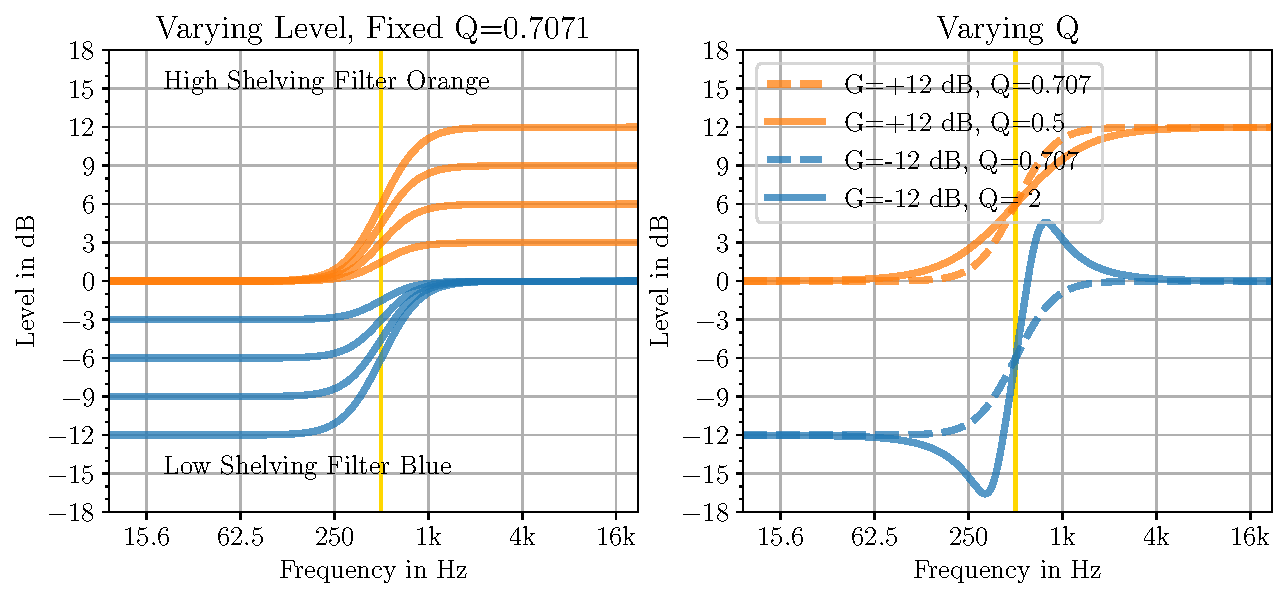
\includegraphics[width=\tw\textwidth]{../graphics/trad-shv-eqs.pdf}
\caption{Typical 2nd order shelving filter with cutoff frequency 500 Hz defined
at mid-level.\\
Slope and transition bandwidth is linked to chosen shelving level and Q-factor.}
\label{fig:trad-shv-eqs}
\end{figure}
\end{frame}
%
%
%
\begin{frame}{Higher Order Shelving Filter Designs}
\begin{figure}
\captionsetup{width=.55\linewidth}
%\includegraphics[width=\tw\textwidth]{McGrath_AES117_Fig19.png}
we don't have copyright, please cf. Figure 19
\caption{[McGrath, Baird \& Jackson, 2004, 117th AES Conv.]\\
Approximation of a shelving filter transition band with PEQ biquads.
%Higher order shelving filter design with cascade of parametric
%equalizers.
}
\label{fig:holters2006-higher-order-shelving}
\end{figure}
\end{frame}
%
%
%
\begin{frame}{Higher Order Shelving Filter Designs}
\begin{center}
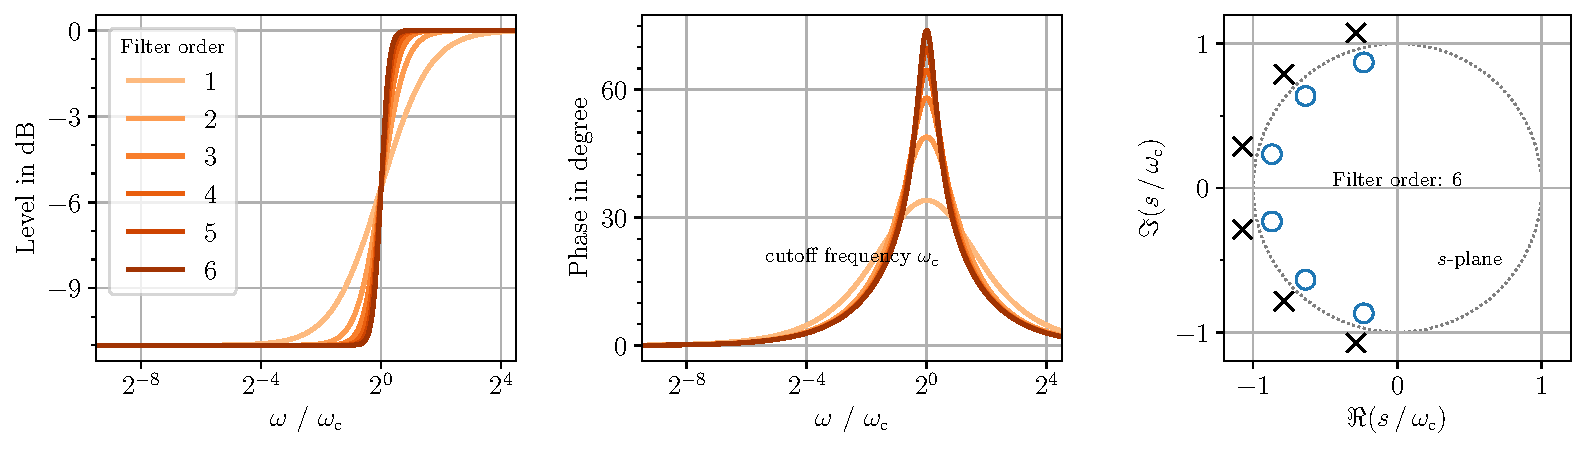
\includegraphics[width=\tw\textwidth]{../graphics/holters2006-higher-order-shelving_slides.pdf}

[Holters \& Z{\"o}lzer, 2006, 120th AES Conv.] Butterworth
alignment of poles and zeros,
cf. [US patent: \#9 722 560]
\end{center}
%
\begin{center}
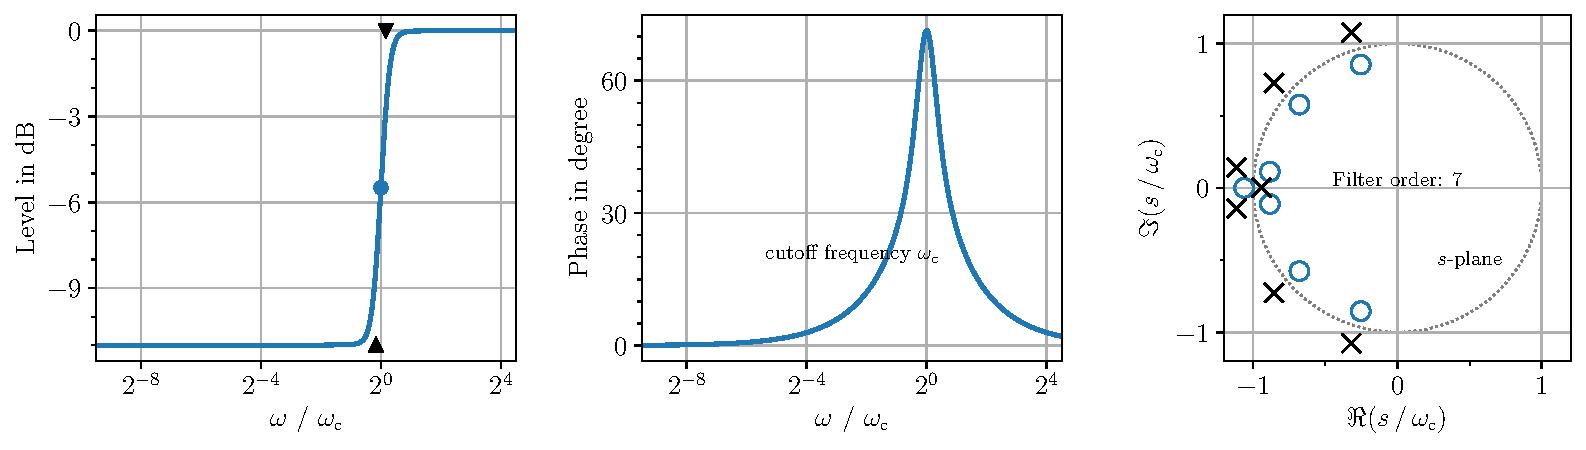
\includegraphics[width=\tw\textwidth]{../graphics/eastty-BW0.3oct-Gd-11dB_slides.pdf}

[Eastty, 2008, 125th AES Conv.] Idea refinement and explicit control of transition
band, cf. [US patent \#9 203 366]

\end{center}
\end{frame}
%
%
%
\section{Proposal}
\begin{frame}{Proposed: Shelving Filter Cascade}
Idea: \textbf{Cascade} of 1st / 2nd order low / high shelving filters to create
\textbf{adjustable transition band}.
%Idea: Cascade of 1st/2nd order low/high shelving filters to create
%higher order shelving filter with adjustable transition band.

Logarithmic alignment due to filter characteristics in log-log domain, also
meaningful for human hearing.
\begin{figure}
\captionsetup{width=.6\linewidth}
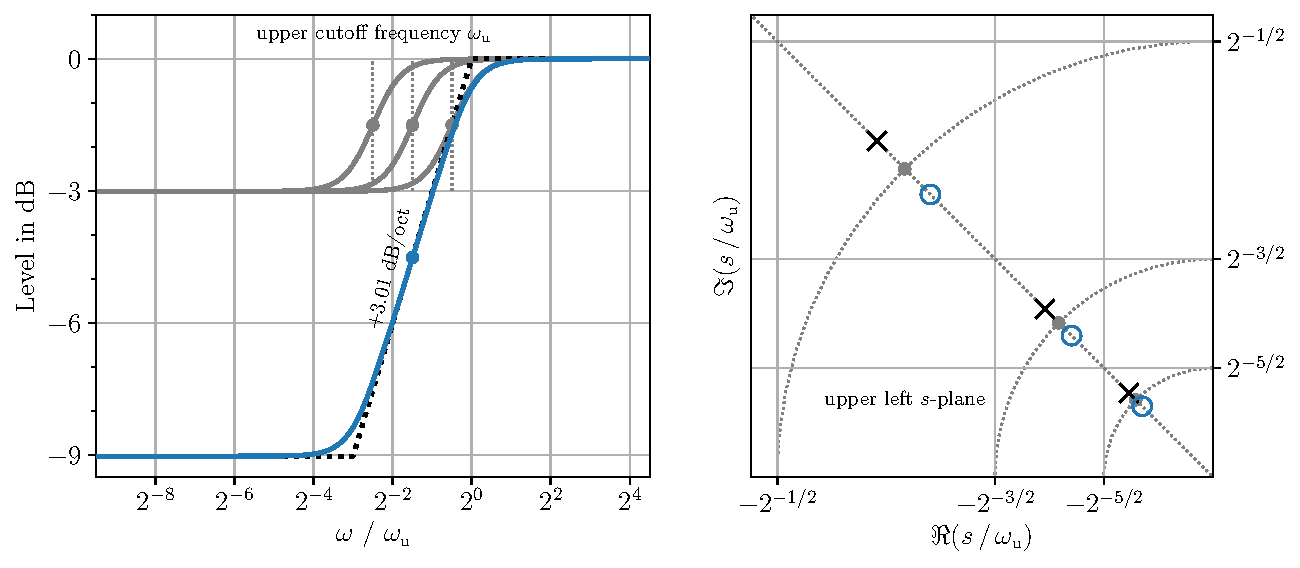
\includegraphics[width=\tw\textwidth]{../graphics/biquad-and-pzmap_slides.pdf}
\caption{[Schultz, Hahn, Spors, 2020, 148th AES Conv.]
Example: $+3\,\mathrm{dB/oct}$ slope and $-9\,\mathrm{dB}$ shelving gain
achieved by one octave spacing of three biquads.}
\label{fig:biquad-and-pzmap}
\end{figure}
\end{frame}
%
%
%
\begin{frame}{Proposed: Shelving Filter Cascade}
Idea: Cascade of 1st / 2nd order low / high shelving filters to create
adjustable transition band:

\small
\textbf{upper cutoff frequency} $\omega_\mathrm{u}>0$ in $\mathrm{rad/s}$,

\textbf{shelving level} $G$ in $\mathrm{dB}$,\quad
\textbf{slope} $\chi$ in $\mathrm{dB/octave}$,\quad
\textbf{bandwidth} $\beta>0$ in $\mathrm{octaves}$
\normalsize
\begin{equation*}
G = \mp\,\beta \cdot \chi
\end{equation*}
%
%
%
\begin{figure}
\centering
\subcaptionbox{
each shelving biquad with mid-level cutoff frequency $\omega_{\mathrm{c},\mu}$.
\label{Fig:1b}
}
{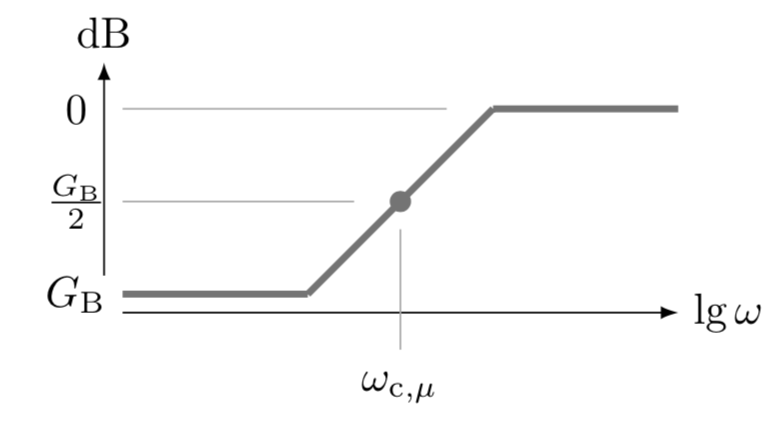
\includegraphics[width=0.3\textwidth]{Fig1b.png}}
\subcaptionbox{
shelving filter cascade with lower / upper cutoff frequency $\omega_\mathrm{l/u}$.
\label{Fig:1c}
}
{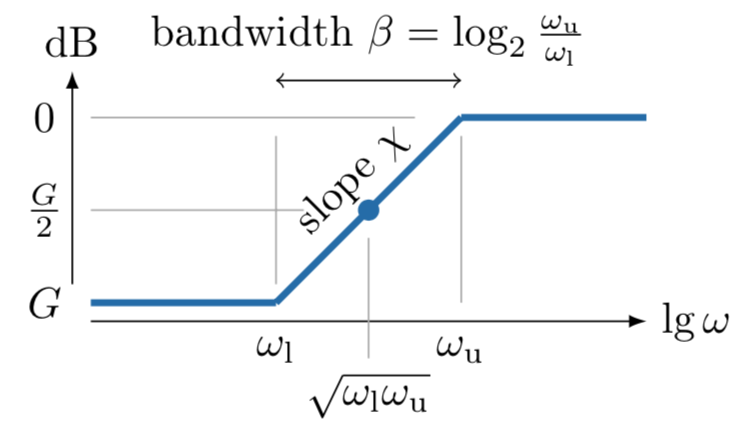
\includegraphics[width=0.3\textwidth]{Fig1c.png}}
\caption{Parameters of (a) shelving biquad and (b) shelving filter
cascade.}\label{Fig:1}
\end{figure}
\end{frame}
%
%
%
\section{Analog Filter Properties}
\begin{frame}{Fixed Level with Varied Slope or Bandwidth}
\begin{figure}
\captionsetup{width=.65\linewidth}
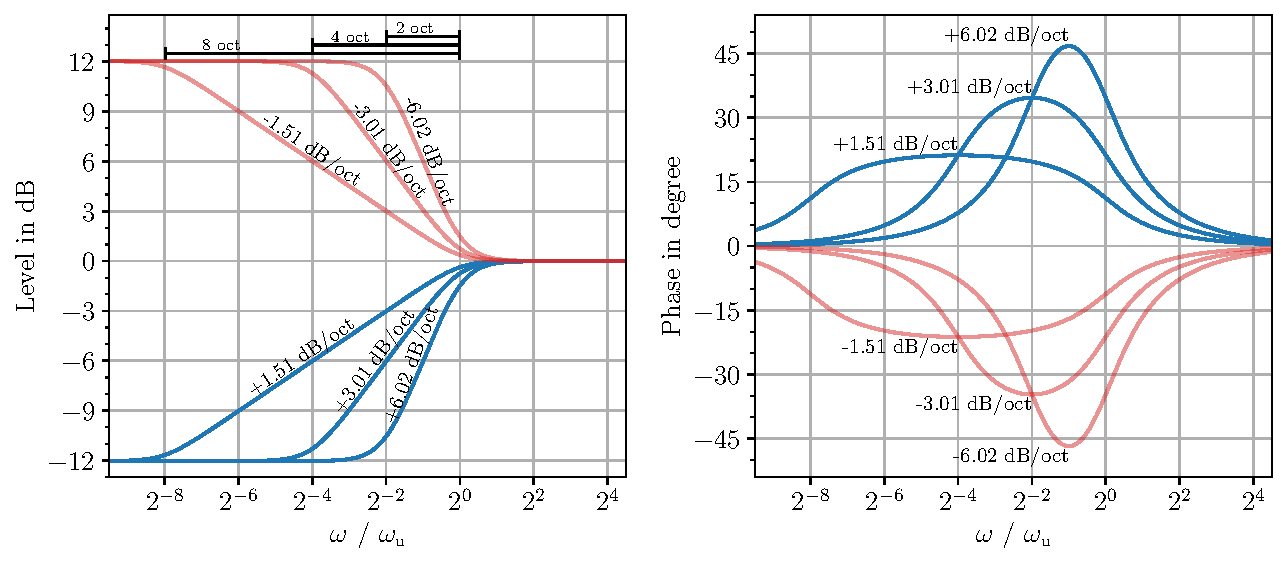
\includegraphics[width=\tw\textwidth]{../graphics/low-shelving-filter-varying-slope.pdf}
\caption{Fixed shelving level $G=\pm 12\,\mathrm{dB}$.\\
Varied slope $\chi$ in $\mathrm{dB/oct}$ with resulting bandwidth $\beta$ in
$\mathrm{oct}$ or vice versa.}
\label{fig:low-shelving-filter-varying-slope}
\end{figure}
%3 biquads per octave
% \footnotesize
% upper cutoff frequency $\omega_\mathrm{u}>0$ in $\mathrm{rad/s}$,\quad
% shelving level $G$ in $\mathrm{dB}$,\quad
% slope $\chi$ in $\mathrm{dB/octave}$,\quad
% bandwidth $\beta>0$ in $\mathrm{octaves}$
\end{frame}
%
%
%
\begin{frame}{Fixed Slope with Varied Bandwidth or Level}
\begin{figure}
\captionsetup{width=.65\linewidth}
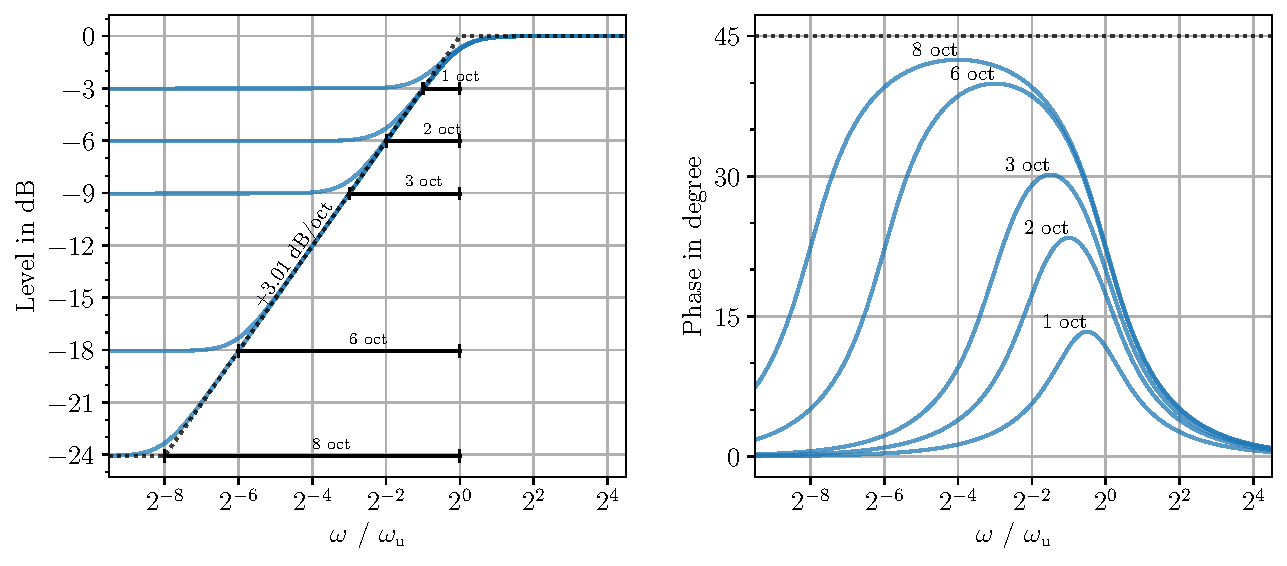
\includegraphics[width=\tw\textwidth]{../graphics/low-shelving-filter-varying-bandwidth.pdf}
\caption{Fixed slope $\chi = 3\,\mathrm{dB/oct.}$\\Varied bandwidth $\beta$
in $\mathrm{oct}$, resulting shelving level $G$ in $\mathrm{dB}$ or vice versa.}
\label{fig:low-shelving-filter-varying-bandwidth}
\end{figure}
% \footnotesize
% upper cutoff frequency $\omega_\mathrm{u}>0$ in $\mathrm{rad/s}$,\quad
% shelving level $G$ in $\mathrm{dB}$,\quad
% slope $\chi$ in $\mathrm{dB/octave}$,\quad
% bandwidth $\beta>0$ in $\mathrm{octaves}$
\end{frame}
%
%
%
\begin{frame}{Fixed Bandwidth with Varied Level or Slope}
\begin{figure}
\captionsetup{width=.65\linewidth}
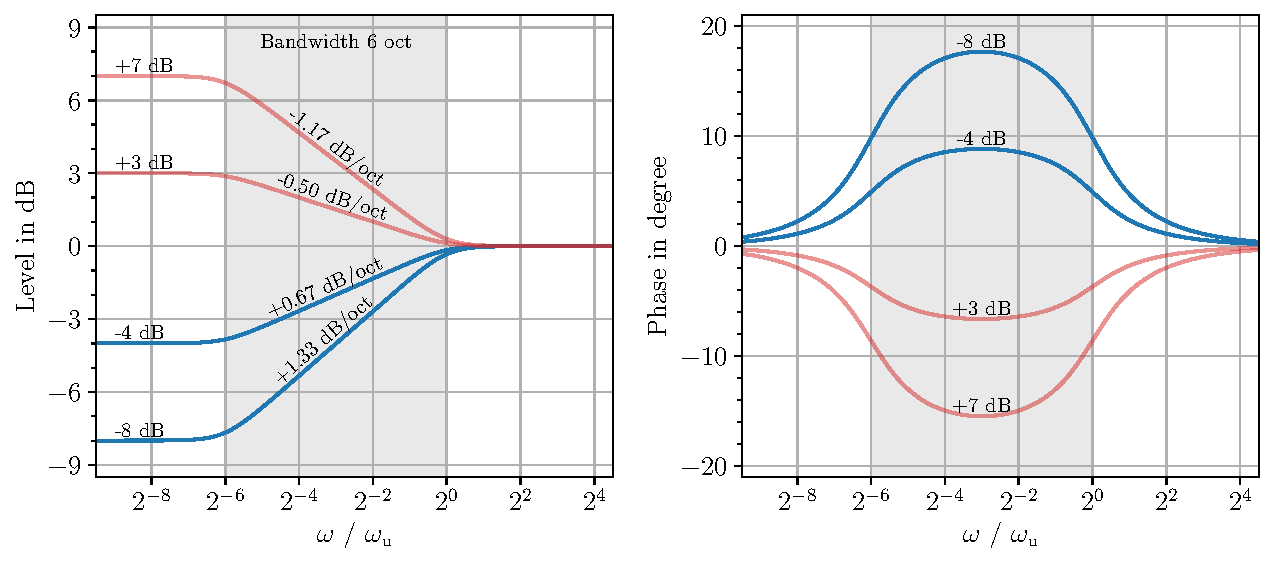
\includegraphics[width=\tw\textwidth]{../graphics/low-shelving-filter-varying-gain.pdf}
\caption{Fixed bandwidth $\beta=6\,\mathrm{oct}$.\\Varied shelving level $G$ in
$\mathrm{dB}$, resulting slope $\chi$ in $\mathrm{dB/oct}$ or vice versa.}
\label{fig:low-shelving-filter-varying-gain}
\end{figure}
% \footnotesize
% upper cutoff frequency $\omega_\mathrm{u}>0$ in $\mathrm{rad/s}$,\quad
% shelving level $G$ in $\mathrm{dB}$,\quad
% slope $\chi$ in $\mathrm{dB/octave}$,\quad
% bandwidth $\beta>0$ in $\mathrm{octaves}$
\end{frame}
%
%
%
\section{Constraints / Limitations}
\begin{frame}{Constraint: Discrete Steps for Shelving Level}
\begin{figure}
\captionsetup{width=.78\linewidth}
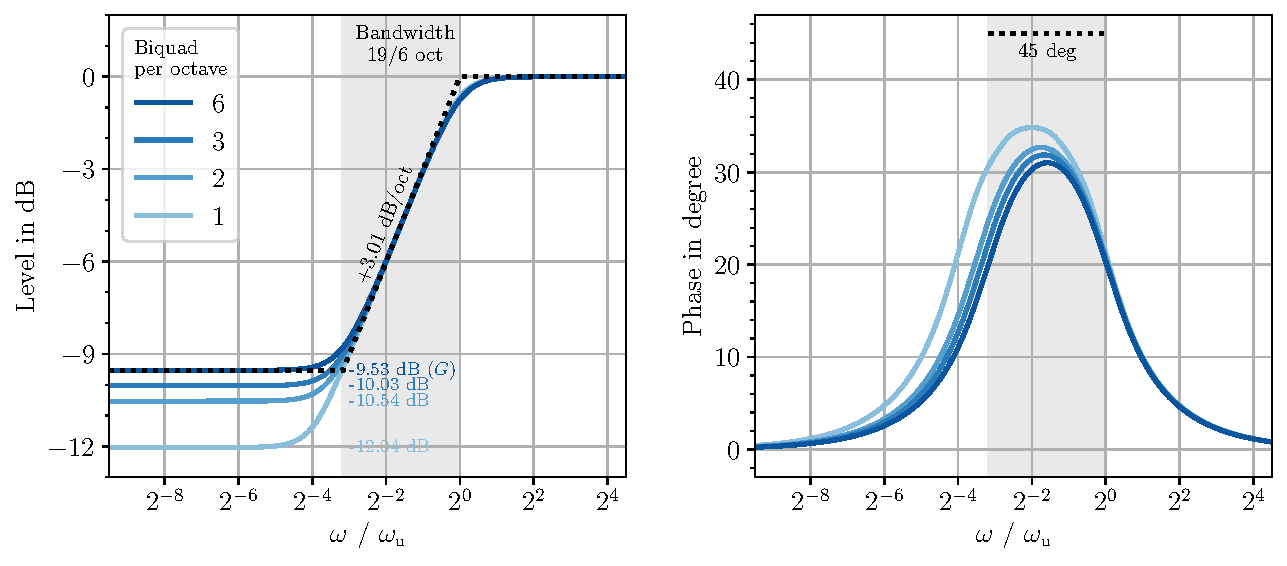
\includegraphics[width=\tw\textwidth]{../graphics/gain-error.pdf}
\caption{The resulting shelving level deviates from $G$ for less than $N_O=6$
biquads per octave.\\
Slope $\chi = 3\,\mathrm{dB/oct}$ and shelving
level $G=-\frac{19}{6}\chi \approx - 9.5\,\mathrm{dB}$\\yields bandwidth
$\beta = 19/6\,\mathrm{oct}$.
}
\label{fig:gain-error}
\end{figure}
\end{frame}
%
%
%
\begin{frame}{Constraint: Ripple Along Transition Slope}
\begin{figure}
\captionsetup{width=.6\linewidth}
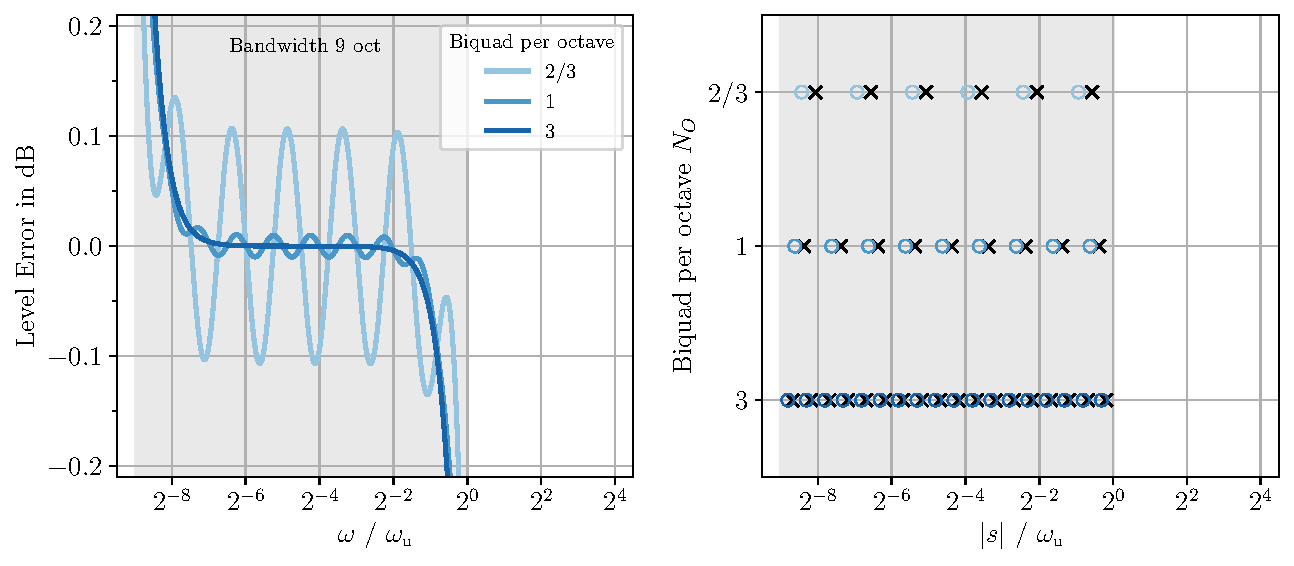
\includegraphics[width=\tw\textwidth]{../graphics/ripple-and-zp-frequency.pdf}
\caption{
Left: Deviation $20\lg|H(\omega)|-20\lg|H_\mathrm{ideal\,slope}(\omega)|$.\\
Right: distribution of poles (x) and zeros (o).\\
$\beta=9\,\mathrm{oct}$,
$G=-10\lg(2)\approx -3\,\mathrm{dB}$ yields\\
$\chi =  \frac{10}{9}\lg(2) \approx + 0.3345\,\mathrm{dB/oct}$.
}
\label{fig:ripple-and-zp-frequency}
\end{figure}
\end{frame}
%
%
%
\section{Digital Filter}
\begin{frame}{Discrete-Time Filter Design}
Straightforward design with bilinear or matched-$z$ transform of biquads
as long as\\
upper cutoff frequency $f_\mathrm{u}$ much smaller than sampling frequency $f_\mathrm{s}$.
\begin{figure}
\captionsetup{width=.6\linewidth}
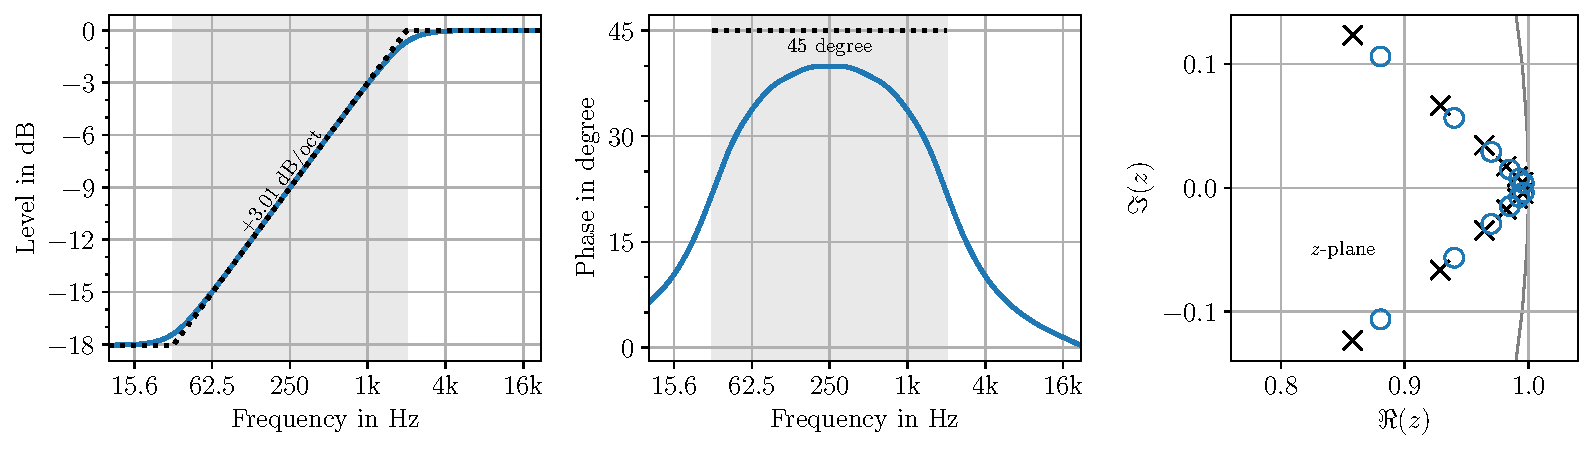
\includegraphics[width=\tw\textwidth]{../graphics/digital-3db-per-octave-shelving-filter_slides.pdf}
\caption{Digital filter design with bilinear transform, cascade of 6 biquads.\\
$3\,\mathrm{dB/oct}$ slope over a $6\,\mathrm{oct}$ bandwidth,\\
$f_\mathrm{u}=2\mathrm{kHz}$, $f_\mathrm{s}=48\,\mathrm{kHz}$, $N_O=1$ biquad per
octave.}
\label{fig:digital-3db-per-octave-shelving-filter}
\end{figure}
\end{frame}










\section{Summary}
%
\begin{frame}{Summary}
\begin{itemize}
  \item Proposing a shelving filter with adjustable
  %cutoff frequency and\\two
  %of three
  parameters
  %adjustable
  : shelving level $G$, \quad bandwidth $\beta$, \quad
  slope $\chi$
  \begin{center}
  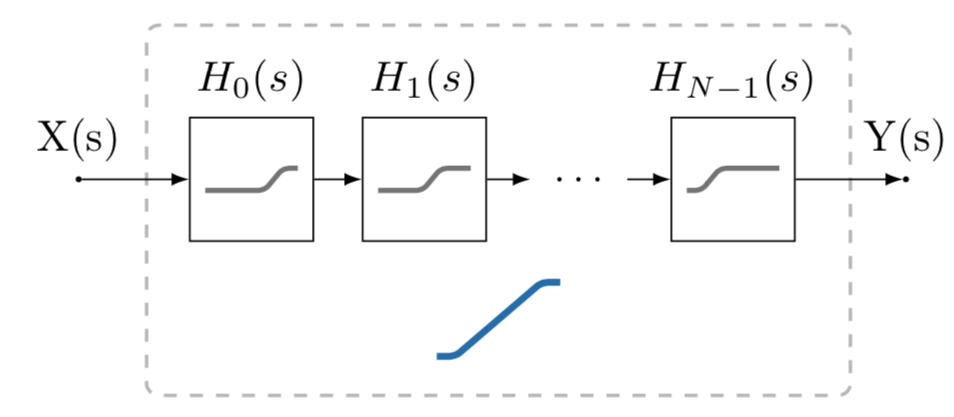
\includegraphics[width=0.33\textwidth,trim=7.5cm 0 0 0]{Fig1a.png}
  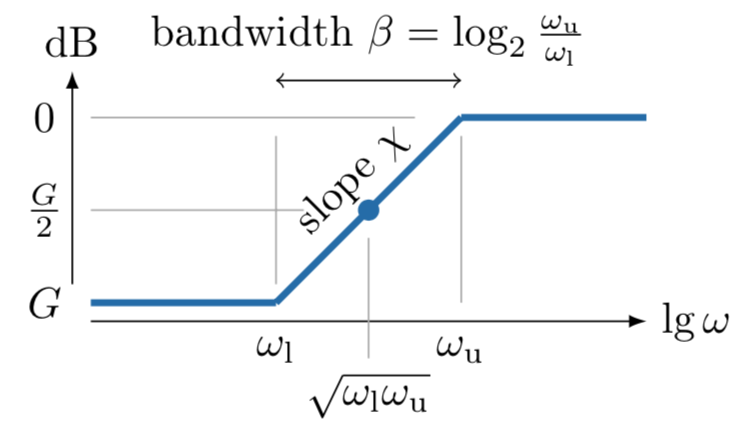
\includegraphics[width=0.33\textwidth,trim=0 0 0 0]{Fig1c.png}
  \end{center}
\item Cascade of 2nd order shelving filters, logarithmically spaced along frequency
\item Limitations are not severe but design must be carefully adapted to specific
target application, i.e. choosing appropriate number of biquads per octave and
the total amount of biquads
\item Potential applications: line array equalizers, audio mixing and production,
sound field synthesis pre-filters, equal loudness contour equalizers
\end{itemize}






\end{frame}
\end{document}
